
%%%%%%%%%%%%%%%%%%%%%%%%%%%%%%%%%%%%%%%%%%%%%%%%%%%%%%%%%%%%%%%
% EDITORIAL SECTION
%
\documentclass{PSAIE}%
\begin{document}%
\PSAIEHeadFirst{10}{1}{1}{3}%
%
% END OF EDITORIAL SECTION
%%%%%%%%%%%%%%%%%%%%%%%%%%%%%%%%%%%%%%%%%%%%%%%%%%%%%%%%%%%%%%%%


% Please give a short title for the running head
\fancyhead[CO]{\PSAIEheader{Short title for the running head}}
% Short list of authors for the running head
\fancyhead[CE]{\PSAIEheader{L. Kov\'acs and A. Ag\'ardi}}
\fancyfoot{}

%The title of your paper
\noindent\PSAIEtitle{This is the Full Title of the Article}

%Data for the first author
\noindent\PSAIEauthor{L\'aszl\'o Kov\'acs}% Authors name for the first author
{University of Miskolc, Hungary\\[0pt]% Address line 1
Department of Information Engineering}% Address line 2
{kovacs@iit.uni-miskolc.hu}% E-mail address for the first author

%Data for the second author
\noindent\PSAIEauthor{Anita Ag\'ardi}% Authors name for the second author
{University of Miskolc, Hungary\\[0pt]% Address line 1
Department of Automation}% Address line 2
{agardianita@iit.uni-miskolc.hu}% E-mail address for the second author

\noindent\PSAIEreceived{\today}

\noindent\PSAIEabstract{This paper is a template for those authors
who wish to prepare their manuscript to be published in
\emph{Production Systems and Information Engineering} by using the
\emph{amsart} document class. You can reedit the text of this
paper and the corresponding \emph{bib} file in order to obtain
your manuscript.}

\noindent\PSAIEkey{keyword1, keyword2}

%%%%%%%%%%%%%%%%%%%%%%%%%%%%%%%%%%%%%%%%%%%%%%%%%%%%%%%%%%%%%%%

\section{Aims and Scope of the Publication}

\noindent The aim of the journal is to publish high quality
research papers connected to both production systems and
information engineering at the same time. Special emphasis is
given to articles on the theoretical models and methods, as well
as practical applications of discrete production processes
including new (or partially new) software tools. Using a new term
proposed in special literature in the nineties, the main profile
of this journal is Production Information Engineering.

\paragraph{Frequency of the journal} One volume per year is planned.

\section{Instructions for Authors}

\subsection{Manuscript Submission}

\noindent Manuscripts should be submitted to the Editor-in-Chief,
Prof. L\'aszl\'o \scshape{Kov\'acs}\upshape, or to the technical secretary Anita Ag\'ardi, who is responsible for preparing the manuscripts for printing:
\begin{itemize}
\item[--] L\'aszl\'o \scshape{Kov\'acs}\upshape :
kovacs@iit.uni-miskolc.hu 
\item[--] Anita
\scshape{Ag\'ardi}\upshape : agardianita@iit.uni-miskolc.hu
\end{itemize}
To speed up publication, email submission of \LaTeX\ manuscripts
is strongly recommended. In this case, please also supply the
corresponding PDF file of your paper that matches exactly the
source text.

\subsection{Conditions of Publication}

\noindent Submission of a manuscript implies that the paper has
not been published, nor is being considered for publication
elsewhere, and that a permission for publication, if needed, has
already been obtained from appropriate sources.

\noindent Please note that the editorial board holds the right to
change the format of the manuscript for compliance with the style
of the journal.

\subsection{Manuscript Preparation}

\subsubsection{Template Files}

\noindent Please, download the provided \textbf{PSAIE.zip} file to
obtain all the necessary template files for manuscript
preparation. This package includes:
\begin{list}{--}{\setlength{\itemsep}{2pt}\setlength{\parsep}{0pt}\setlength{\leftmargin}{15mm}}
\item \textbf{PSAIE.cls}: it contains all the default settings.
This file must be included into your \LaTeX\ file and should not
be changed under any circumstances. \item
\textbf{PSAIEsample.tex}: sample \LaTeX\ file -- this is to be
edited \item \textbf{PSAIEbib.bst}: bibliography style file to
prepare your bibliography by using Bib\TeX. Please, do not make
any changes to this file. \item \textbf{PSAIESampleBib.bib}:
sample Bib\TeX\ literature database file -- this is to be edited
\item \textbf{cimer-ff.eps}: picture file appearing in the first
page heading of the manuscript
\end{list}

\subsubsection{Graphic Files}

\noindent It is not recommended to use the built-in graphical
facilities of the editors. Please, prepare your figures with
special graphics tools and then include them in your manuscript.

\subsubsection{Note for Scientific Word and Scientific Workplace Users}

\noindent If you use Windows and Scientific Word or Scientific Workplace, please
make sure that you save your \LaTeX\ manuscript as the so-called
Portable \LaTeX. The final manuscript should not contain any
non-standard macros.


\section{Examples}

\noindent Some text and some formula:
\begin{equation}
y_n(t,x)=
\begin{cases}
 f(t,x) & \text{for } (t,x) \in A \cr
f_n(t,x) & \text{for } (t,x) \not\in A.
\end{cases}
\end{equation}

\noindent Some sample references: see
\cite{ChenYhou1992,Paulino1995} or \cite{Gurtin1972}.

\begin{figure}[h!]
\begin{center}
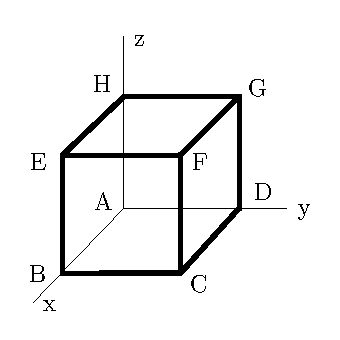
\includegraphics[keepaspectratio,width=4cm]{FigureOne.eps}
\caption{Sample figure}
\end{center}
\end{figure}

\begin{table}[h]
\caption{Sample table}
\begin{tabular}{|l|l|}
\hline \textbf{Name} & \textbf{Email} \\
\hline L. Kov\'acs & kovacs\verb+@+iit.uni-miskolc.hu \\
\hline A. Ag\'ardi & agardianita\verb+@+iit.uni-miskolc.hu \\
\hline
\end{tabular}
\end{table}


\section*{Acknowledgements} % A simple way to write acknowledgements
\noindent
The authors express their gratitude to the XXX Institute at YYY for
their hospitality, etc.

%%%%%%%%%%%%%%%%%%%%%%%%%%%%%%%%%%%%%%%%%%%%%%%%%%%%%%%%%%%%%%%%%%
%\begin{thebibliography}{99}

%\bibitem{ChenYhou1992}
%\textsc{Chen, G.} and \textsc{Yhou, J.}: \emph{Boundary {E}lement
%{M}ethods}. Academic Press Limitid, 24-28 Oval Road, London, NW1
%7DX, 1992, ISBN 0-1-170840-X.

%\bibitem{Gurtin1972}
%\textsc{Gurtin, M.~E.}: The {L}inear {T}heory of {E}lasticity. In
%S.~Fl\"ugge (ed.), \emph{{H}andbuch der {P}hysik,
%{F}estk\"{o}rpermechanik}, vol.~2, pp. 17, 57--60, 163--164,
%Springer Verlag, Berlin, Heidleberg, NewYork, 1st edn., 1972.

%\bibitem{Paulino1995}
%\textsc{Paulino, G.~H.}: \emph{Novel {F}ormulations of the
%{B}oundary {E}lement {M}ethod for {F}racture {M}echanics and
%{E}rror {E}stimation}. Ph. {D}. {D}issertation, Cornel University,
%Ithaca, NY, USA, 1995.

%\end{thebibliography}
%%%%%%%%%%%%%%%%%%%%%%%%%%%%%%%%%%%%%%%%%%%%%%%%%%%%%%%%%%%%%%%%%%%%

%%% If using BibTeX, "thebibliography" environment %%%
%%% should be replaced by the following commands  %%%
\bibliographystyle{PSAIEbib}  %Bibliography style file (*.bst)
\bibliography{PSAIESampleBib} %Bibliography file (*.bib)

%%%%%%%%%%%%%%%%%%%%%%%%%%%%%%%%%%%%%%%%%%%%%%%%%%%%%%%%%%%%%%%%%%%%
\end{document}%

